\documentclass[../main.tex]{subfiles}

\begin{document}

\section{Experimental Setup}
\justify

This chapter describes the concrete setup that turns the approach in the previous chapter into a working system. It covers the simulator, the corridor used for training and evaluation, the tree spawning, the camera and depth pipeline, the asymmetric actor--critic policy and action space, the simulation and real-world evaluation protocols, and the physical drone built to match the simulated platform. Figure~\ref{fig:exp_overview} provides a high-level view of the full experimental setup.

\begin{figure}[h]
  \centering
  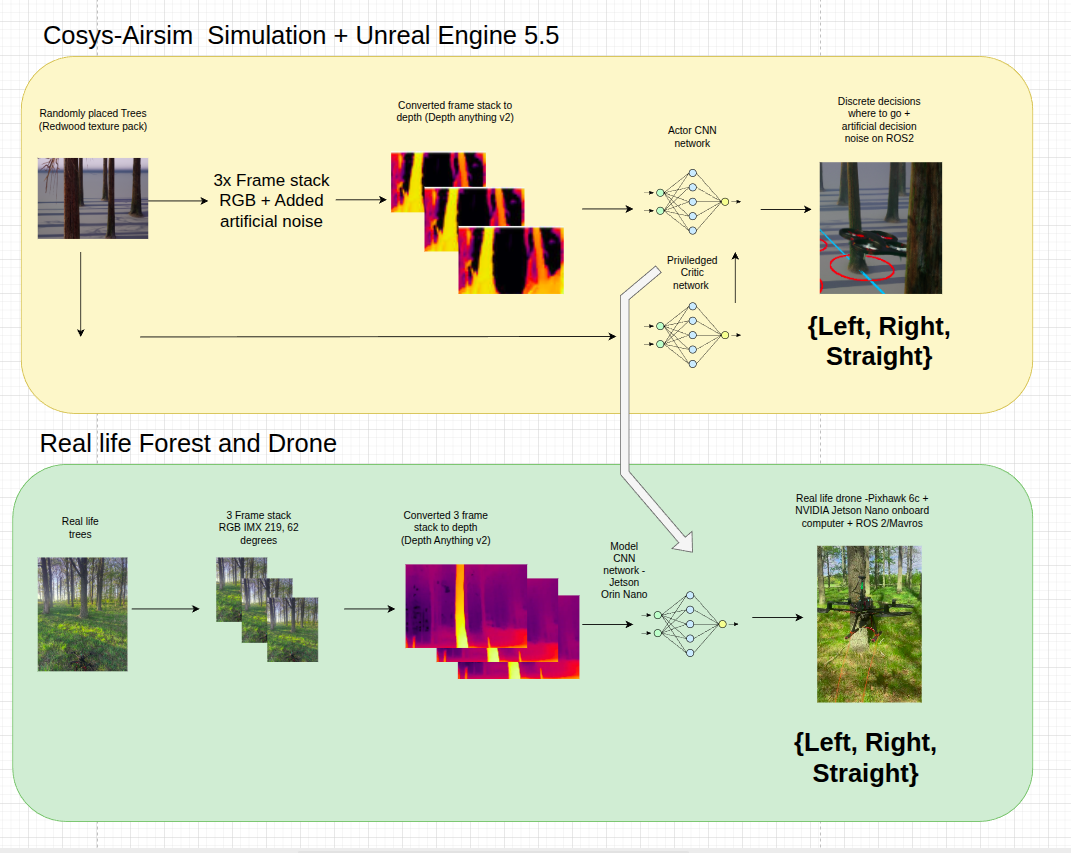
\includegraphics[width=1\textwidth]{figures/methodology.png}
  \caption{High-level overview of the experimental setup, showing the simulation environment, the onboard inference pipeline, and the real-world deployment platform.}
  \label{fig:exp_overview}
\end{figure}

\subsection{Simulation Environment}

All training and evaluation in simulation is run in \textit{Cosys-AirSim}, a community fork of \textit{Microsoft AirSim} \cite{Kabas2022}, on top of \textit{Unreal Engine 5.5}. Cosys-AirSim is used specifically because it exposes \texttt{simSetObjectPose} and \texttt{simSetObjectScale}, which allow tree positions, angles, and sizes to be changed between episodes without reloading the scene -- this is what makes the heavy domain randomisation in this work practical. Figure~\ref{fig:sim_forest} shows the simulated forest scene.

\begin{figure}[h]
  \centering
  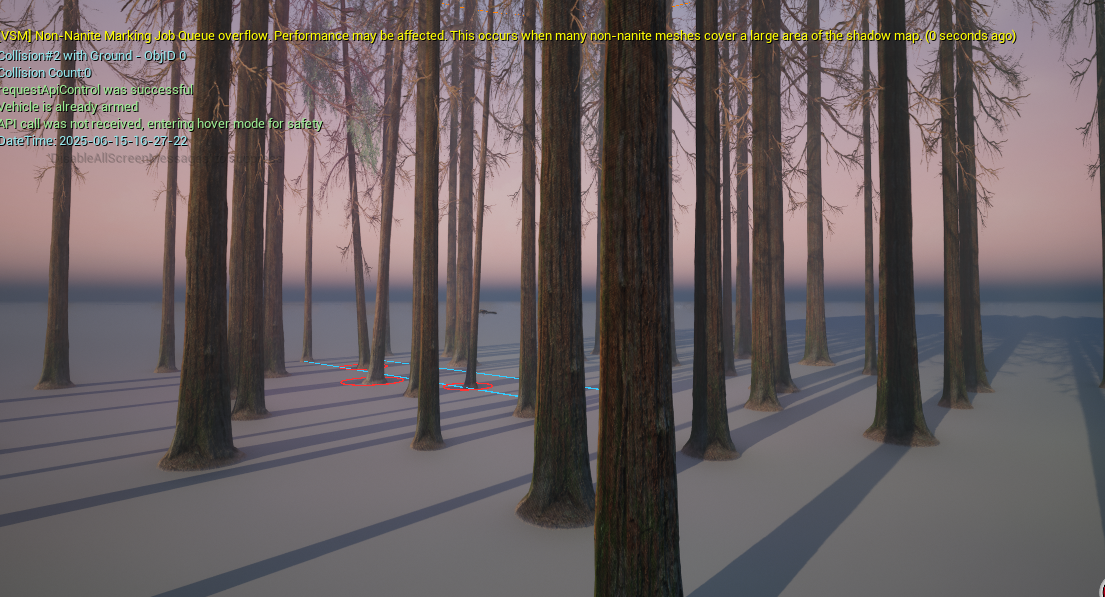
\includegraphics[width=1\textwidth]{figures/sim-forest.png}
  \caption{The simulated forest corridor in Cosys-AirSim, rendered in Unreal Engine 5.5 using a redwood texture pack.}
  \label{fig:sim_forest}
\end{figure}

The simulated forest is a 15\,m long, 4\,m wide corridor placed inside an Unreal scene built from a redwood texture pack. Since this thesis evaluates on naked tree trunks only, the specific tree species or texture is not central to the method; the texture pack provides a visually consistent set of trunks while still varying in shape and bark detail. Trees inside the corridor act as obstacles and trees placed outside the corridor act as visual background.


\subsection{Tree Spawning and Difficulty Stages}

The training curriculum has two difficulty stages, both inside the same 15\,m corridor:

\begin{itemize}
  \item \textbf{Sparse} -- 2 trees inside the corridor, placed at random positions.
  \item \textbf{Dense} -- 3 trees inside the corridor, placed at random positions.
\end{itemize}

Across both stages, the in-corridor trees and the surrounding background trees are spawned in a random order, with random angles (tilted up to roughly $\pm 30^{\circ}$--$45^{\circ}$ off vertical) and random trunk thickness drawn within stage-specific bounds. Background trees outside the corridor are placed throughout the visible area so that domain randomisation does not just affect the obstacles themselves but also the visual context the camera sees \cite{Loquercio2019}.


\subsection{Camera, Frame Stack, and Depth Pipeline}

The simulated camera matches the physical sensor exactly. It is a single forward-facing camera with a $62^{\circ}$ field of view, the same FOV as the Arducam camera mounted on the real drone, so there is no FOV mismatch between simulation and reality \cite{Loquercio2019,Zhao2020}. Each captured frame is resized to $126 \times 224$\,px and pushed through Depth Anything V2 \cite{Yang2024DepthAnythingV2}, which produces a depth image at the same resolution.

The policy does not see a single frame. It sees a 3-frame stack of depth images, with frames sampled 5 control steps apart; at the $\sim$10\,Hz control rate of the agent, this means each new depth frame is roughly $0.5$\,s and $\sim 0.5$\,m of forward motion older than the next, so the 3-frame stack covers about a metre of recent motion. This gives the network implicit motion information without any optical-flow computation \cite{Kabas2022}.


To make the policy robust to the differences between simulation and reality, several types of randomisation and noise are applied to this pipeline at training time:

\begin{itemize}
  \item \textbf{Image noise.} Per-frame Gaussian noise with standard deviation drawn uniformly from $[0.01,\,0.03]$, plus per-episode brightness and contrast jitter \cite{Loquercio2019,Zhao2020}.
  \item \textbf{Motion blur.} Directional smear scaled by the recent lateral action, replicating the motion blur of a real camera during sharp avoidance manoeuvres.
  \item \textbf{Camera-mounting jitter.} The simulated camera is offset by a small random rotation per episode, replicating imperfect mounting on the real airframe.
  \item \textbf{Spawn yaw jitter.} The drone does not always start perfectly aligned with the corridor axis.
  \item \textbf{Velocity drift.} A small random drift (up to $0.3$\,m/s) is added to baseline velocities.
  \item \textbf{Inference / pipeline delay.} The action chosen at step $t$ is not executed until step $t+\Delta$, with $\Delta$ randomly fixed to 1 or 2 control steps ($\sim$100--200\,ms) per episode, replicating real-world Depth Anything inference latency on the onboard Jetson.
  \item \textbf{Action noise.} Small noise is also injected into the discrete-action selection during training to keep the policy from over-fitting to perfect, instantaneous responses.
\end{itemize}

These noise sources are derived from the sim-to-real strategies in \cite{Loquercio2019,Zhao2020,Salvato2021}, with the specific configuration of pipeline delay and motion blur tailored to the Depth Anything inference profile observed on the target Jetson hardware. Figure~\ref{fig:sim_camera} shows an example of the simulated camera output after augmentation.

\begin{figure}[H]
  \centering
  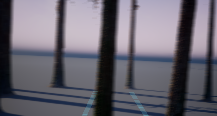
\includegraphics[width=0.65\textwidth]{figures/sim-camera.png}
  \caption{Example simulated camera frame after noise augmentation, showing the $62^{\circ}$ FOV and the Depth Anything V2 depth map alongside the RGB input.}
  \label{fig:sim_camera}
\end{figure}
\subsection{Reward, Corridor Constraint, and Episode Termination}

The reward function is the dense-plus-sparse design described in Section~3 (forward-progress shaping, time penalty, centerline bonus, lateral penalty, terminal goal/collision/efficiency rewards \cite{Schulman2017,Kabas2022,Loquercio2019,DelCol2025}). On top of that, the corridor itself is a hard constraint: the drone is allowed to move freely within the $15\times4$\,m corridor, but any lateral excursion outside the corridor immediately ends the episode.

An episode therefore ends in one of three ways: \textit{success} (the drone reaches the end of the corridor), \textit{collision} (any contact with a tree), or \textit{out-of-bounds} (the drone leaves the corridor sideways). All three trigger a respawn at the corridor entrance for the next episode. This respawn-on-failure / respawn-on-success structure is the same training pattern Kabas \cite{Kabas2022} used for AirSim corridor episodes and that Loquercio et al.\ \cite{Loquercio2019} used during DAgger-style trajectory recovery. Figure~\ref{fig:sim_corridor_annotated} shows the corridor with its termination boundaries marked.

\begin{figure}[H]
  \centering
  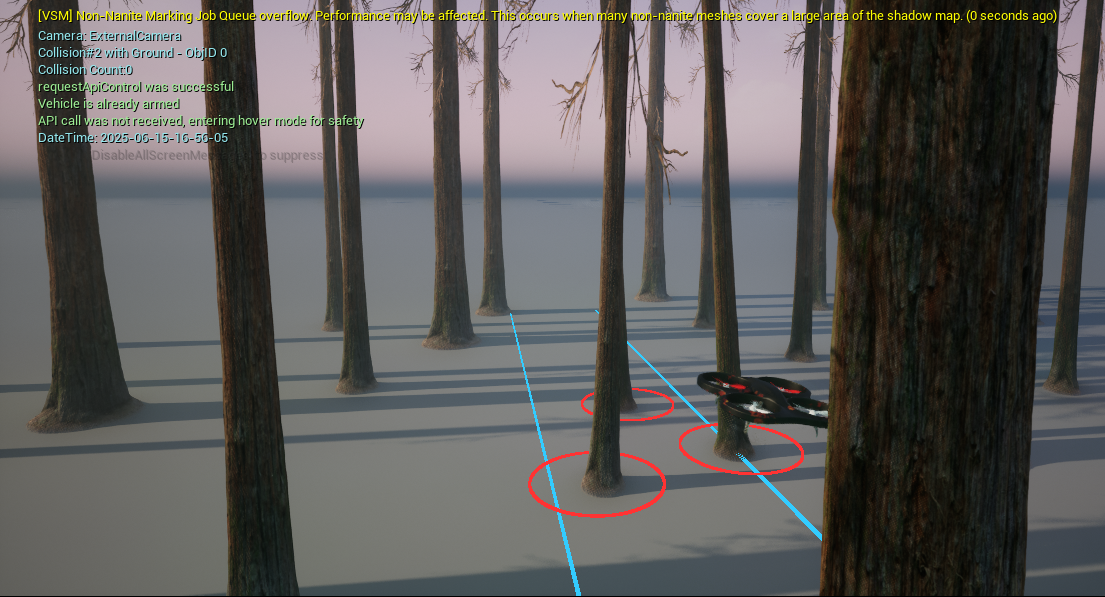
\includegraphics[width=1\textwidth]{figures/sim-corridor.png}
  \caption{The 15\,m\,$\times$\,4\,m simulated corridor with termination boundaries annotated: the corridor end (success), the lateral walls (out-of-bounds), and tree trunks (collision).}
  \label{fig:sim_corridor_annotated}
\end{figure}



\subsection{Asymmetric Actor--Critic and Action Space}

The policy is trained with PPO \cite{Schulman2017} in an asymmetric actor--critic configuration \cite{Pinto2017}. The two networks see different things on purpose:

\begin{itemize}
  \item \textbf{Actor (the student).} Receives only the 3-frame depth stack from the camera. It runs a CNN over those depth images and outputs a categorical distribution over 3 discrete actions. The actor never sees tree positions, drone pose, or any other privileged simulator state.
  \item \textbf{Critic (the teacher).} Receives a 66-dimensional privileged vector containing the drone's position and velocity, the goal location, and the position and scale of up to 20 nearest trees. It does not see any image. Its only job is to provide a high-quality value estimate that the actor can learn from.
\end{itemize}


Because the actor only ever sees what will be available on the real drone (a depth-converted camera image), the policy never becomes dependent on signals that vanish at deployment. Because the critic exploits the full simulator state, it provides a tighter value baseline than an image-only critic could, which is the main argument of the asymmetric setup in Pinto et al.\ \cite{Pinto2017}.

The actor's discrete action space is $\{\text{Left},\ \text{Straight},\ \text{Right}\}$. These map to a velocity command:

\begin{itemize}
  \item \textbf{Straight} -- forward $1.0$\,m/s, lateral $0$\,m/s. Cruise.
  \item \textbf{Left / Right} -- forward $0$\,m/s, lateral $\pm 2.0$\,m/s. Hard avoidance step.
\end{itemize}

The forward-only $1$\,m/s cruise is intentionally conservative for forest flight, while the $\pm 2$\,m/s lateral commit is sharp enough to clear a trunk before the drone passes it. The control loop runs at approximately $10$\,Hz effective decision rate (the $30$\,Hz physics simulation is queried with a frame-skip of 3). This rate is what makes the $\sim$100--200\,ms randomised pipeline delay above realistic.

Yaw is locked to the direction of travel so the camera always faces forward, and altitude is held by an external P-controller, so altitude is not part of the RL action space.



\subsection{Real-World Hardware}

The drone platform used in this thesis was assembled and integrated as part of a parallel Systems Engineering course; the hardware design and component selection are not contributions of this thesis. The following describes the platform as used for the navigation experiments.

The physical drone is a Holybro S500 V2 quadrotor (500\,mm wheelbase, $\sim 1.75$\,kg all-up weight), chosen because its airframe comfortably accommodates the NVIDIA Jetson Orin Nano companion computer used for inference and because its dimensions match the simulated drone in Cosys-AirSim. Compute is split between the Jetson, which runs Depth Anything V2 inference and the PPO policy, and a Pixhawk 6C flight controller (running PX4) which receives velocity commands from the Jetson and produces the actual motor outputs. The Jetson talks to the Pixhawk over MAVLink. The assembled platform is shown in Figure~\ref{fig:real_drone}.

\begin{figure}[H]
  \centering
  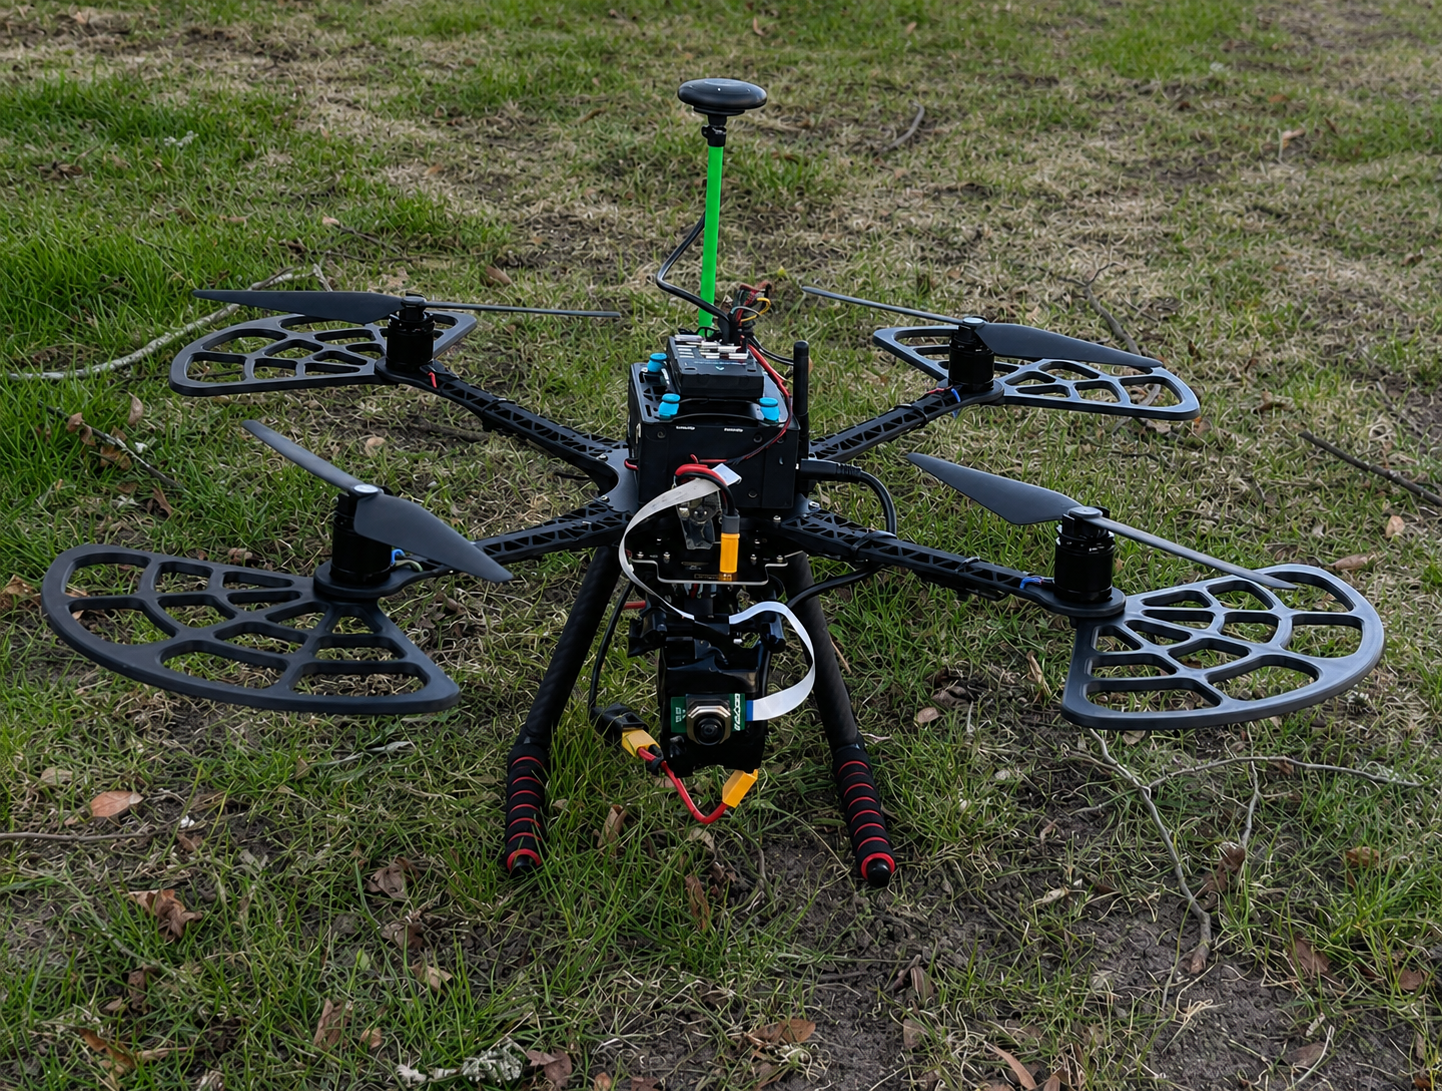
\includegraphics[width=0.8\textwidth]{figures/drone.png}
  \caption{The physical Holybro S500 V2 drone with the Jetson Orin Nano companion computer, Arducam IMX219 camera, and Pixhawk 6C flight controller.}
  \label{fig:real_drone}
\end{figure}
\vspace{1cm}
The camera is an Arducam IMX-series module configured to a $62^{\circ}$ horizontal field of view, the same FOV as the simulated camera. At a unit price of around \$20, it is the cheapest perception sensor on the platform by a wide margin compared with stereo (\$300--800) or LiDAR (\$1{,}000--10{,}000) alternatives \cite{Butt2024,Hrabar2012}. Table \ref{tab:hardware} lists every component.

\begin{table}[H]
    \small
    \centering
    \caption{Physical drone hardware components.}
    \label{tab:hardware}
    \begin{tabular}{p{4cm} p{9cm}}
        \hline\hline
        \rowcolor{lightgray}\textbf{Component} & \textbf{Specification} \\\hline
        Frame & Holybro S500 V2 (500\,mm wheelbase) \\
        \rowcolor{lightlightgray} Flight controller & Pixhawk 6C, PX4 firmware v1.14+ \\
        Companion computer & NVIDIA Jetson Orin Nano (8\,GB) \\
        \rowcolor{lightlightgray} Camera & Arducam IMX477, 100\textdegree{} FOV, 128$\times$128 @ 60\,fps (tuned to 30\,fps) \\
        GPS & Holybro M10 GPS module \\
        \rowcolor{lightlightgray} Telemetry & 433\,MHz SiK radio \\
        Battery & 4S 5000\,mAh LiPo (5--10\,min flight time) \\
        \rowcolor{lightlightgray} Communication & MAVLink via UART \\
        \hline
    \end{tabular}
\end{table}


\subsection{Middleware and Software}

The same middleware stack is used in simulation and on the real drone, which keeps the codebase between the two environments as close to identical as possible. ROS\,2 connects the Jetson to the rest of the system. The camera publishes frames on a ROS\,2 topic, which an inference node consumes, runs through Depth Anything V2 and the PPO policy, and republishes as velocity commands. MAVROS bridges those ROS\,2 commands to MAVLink and into the Pixhawk's velocity-control mode, and the same MAVROS bridge is used in simulation, where the Cosys-AirSim drone exposes a MAVLink-compatible interface. The result is that the inference graph that runs in simulation is the same graph that runs in the real forest -- only the producer of the camera feed differs. The ROS\,2 pipeline is illustrated in Figure~\ref{fig:ros2_pipeline}, and the full software stack is listed in Table~\ref{tab:software}.

\begin{figure}[h]
  \centering
  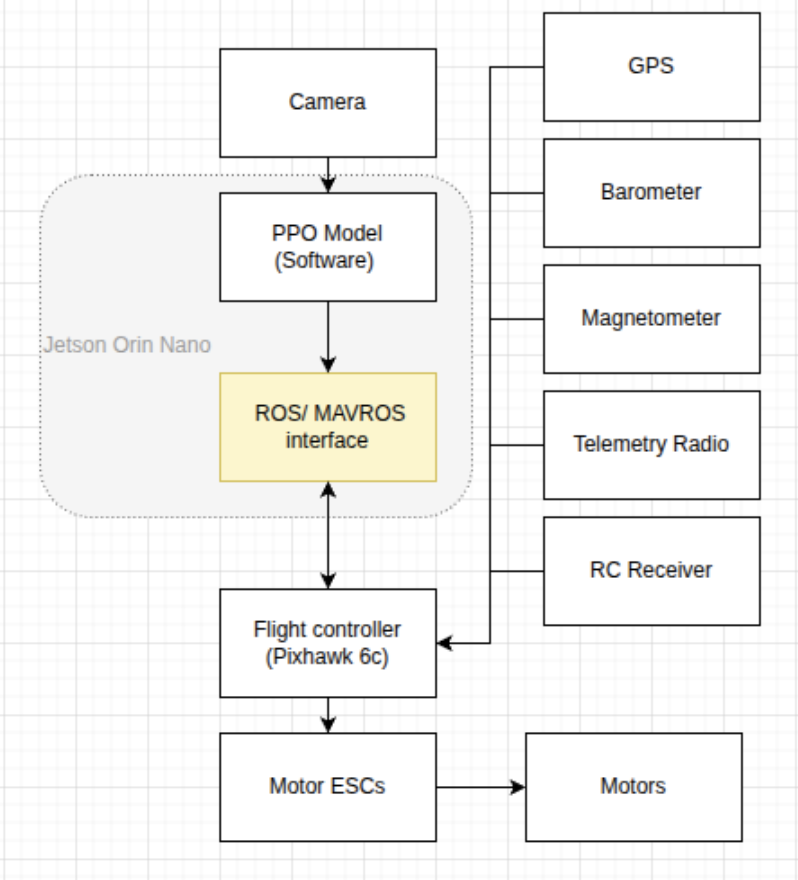
\includegraphics[width=0.45\textwidth]{figures/ros2_pipeline.png}
  \caption{The ROS\,2 inference pipeline: camera frames flow through Depth Anything V2 and the PPO policy node, with velocity commands forwarded to the Pixhawk via MAVROS.}
  \label{fig:ros2_pipeline}
\end{figure}
\vspace{1cm}

\begin{table}[H]
    \small
    \centering
    \caption{Software stack for training and real-world deployment.}
    \label{tab:software}
    \begin{tabular}{p{4cm} p{4cm} p{5.5cm}}
        \hline\hline
        \rowcolor{lightgray}\textbf{Component} & \textbf{Tool} & \textbf{Role} \\\hline
        Simulation environment & Cosys-AirSim + UE 5.5 & Physics, rendering, sensor simulation \\
        \rowcolor{lightlightgray} RL framework & Stable-Baselines3 + PyTorch & PPO training \\
        Image processing & OpenCV & CLAHE preprocessing, image capture \\
        \rowcolor{lightlightgray} Camera interface & ROS2 & Arducam frame streaming to Jetson \\
        Sensor interface & MAVROS & Pixhawk IMU/GPS data to Jetson \\
        \rowcolor{lightlightgray} Flight commands & MAVSDK-Python + MAVLink & Velocity commands to Pixhawk \\
        Inference optimisation & TensorRT & Real-time policy inference on Jetson \\
        \rowcolor{lightlightgray} Ground station & QGroundControl & Telemetry monitoring, safety override \\
        \hline
    \end{tabular}
\end{table}


\subsection{Simulation and Real-World Evaluation}

Simulation and real-world trials follow the same protocol so the two can be compared directly. In simulation, the policy is evaluated under fixed, deterministic conditions with noise and randomisation disabled and the curriculum fixed: 50 episodes in the sparse stage and 50 in the dense stage, giving 100 simulation episodes.

The same policy is then deployed without fine-tuning on the physical drone, with 50 flights per stage conducted in a Swedish forest of naked tree trunks. Each flight is set up in a different section of the forest, so no two episodes use the same tree positions. The real-world stages are not replicas of simulated corridors; instead, they share the same defining criteria: a 15\,m\,$\times$\,4\,m corridor boundary, the same tree count per stage (2 for sparse, 3 for dense), and the same episode success and termination rules. Tree positions and trunk sizes within those boundaries vary naturally between episodes, just as they are randomised in simulation. Real flights run under controlled but realistic outdoor conditions (wind below $3$\,m/s, no precipitation, sufficient daylight). An episode counts as a success, in either environment, if the drone clears the corridor without tree contact, without leaving the corridor laterally, and -- in the real world -- without manual safety override. Figure~\ref{fig:corridor_sxs} shows the simulated and real corridors side by side. Figure~\ref{fig:fpv_sxs} shows the first-person view in both environments, and Figure~\ref{fig:drone_sxs} shows the simulated and physical drone platforms.

\begin{figure}[H]
  \centering
  \begin{minipage}[t]{0.48\textwidth}
    \centering
    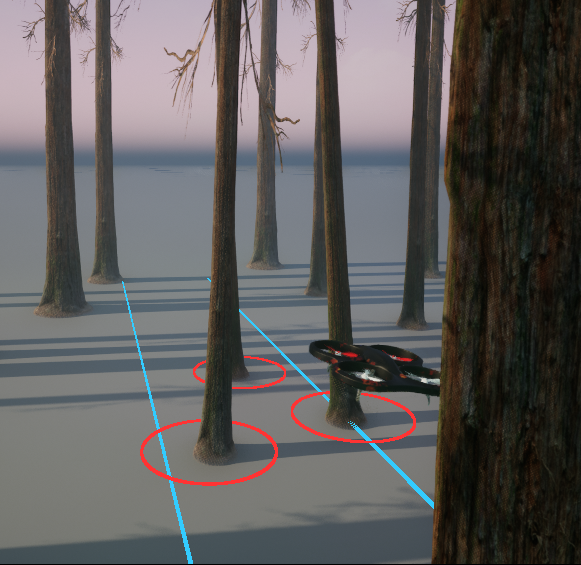
\includegraphics[height=7cm]{figures/sim-corridor-narrow.png}
    \subcaption{Simulated corridor (AirSim).}
  \end{minipage}\hfill
  \begin{minipage}[t]{0.48\textwidth}
    \centering
    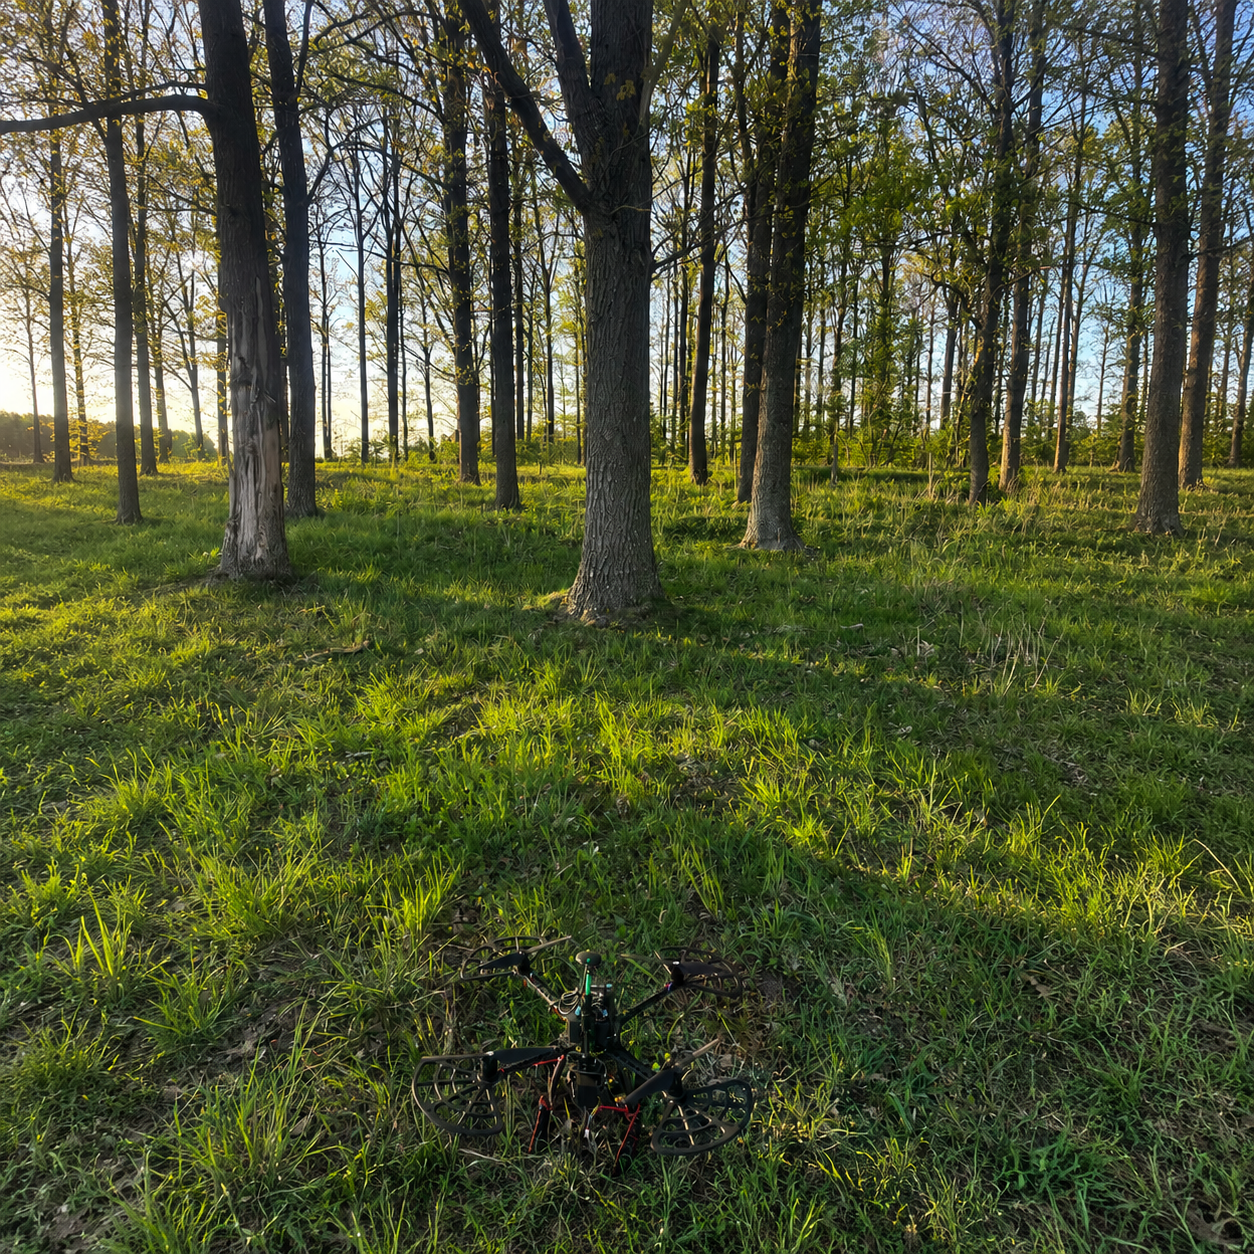
\includegraphics[height=7cm]{figures/real-corridor.png}
    \subcaption{Real Swedish forest corridor.}
  \end{minipage}
  \vspace{1cm}
  \caption{Simulated and real evaluation corridors, side by side.}\label{fig:corridor_sxs}
\end{figure}

\begin{figure}[H]
  \centering
  \begin{minipage}[t]{0.48\textwidth}
    \centering
    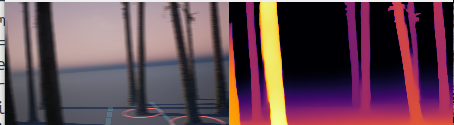
\includegraphics[width=\linewidth]{figures/side-by-side.png}
    \subcaption{Simulated first-person view.}
  \end{minipage}\hfill
  \begin{minipage}[t]{0.48\textwidth}
    \centering
    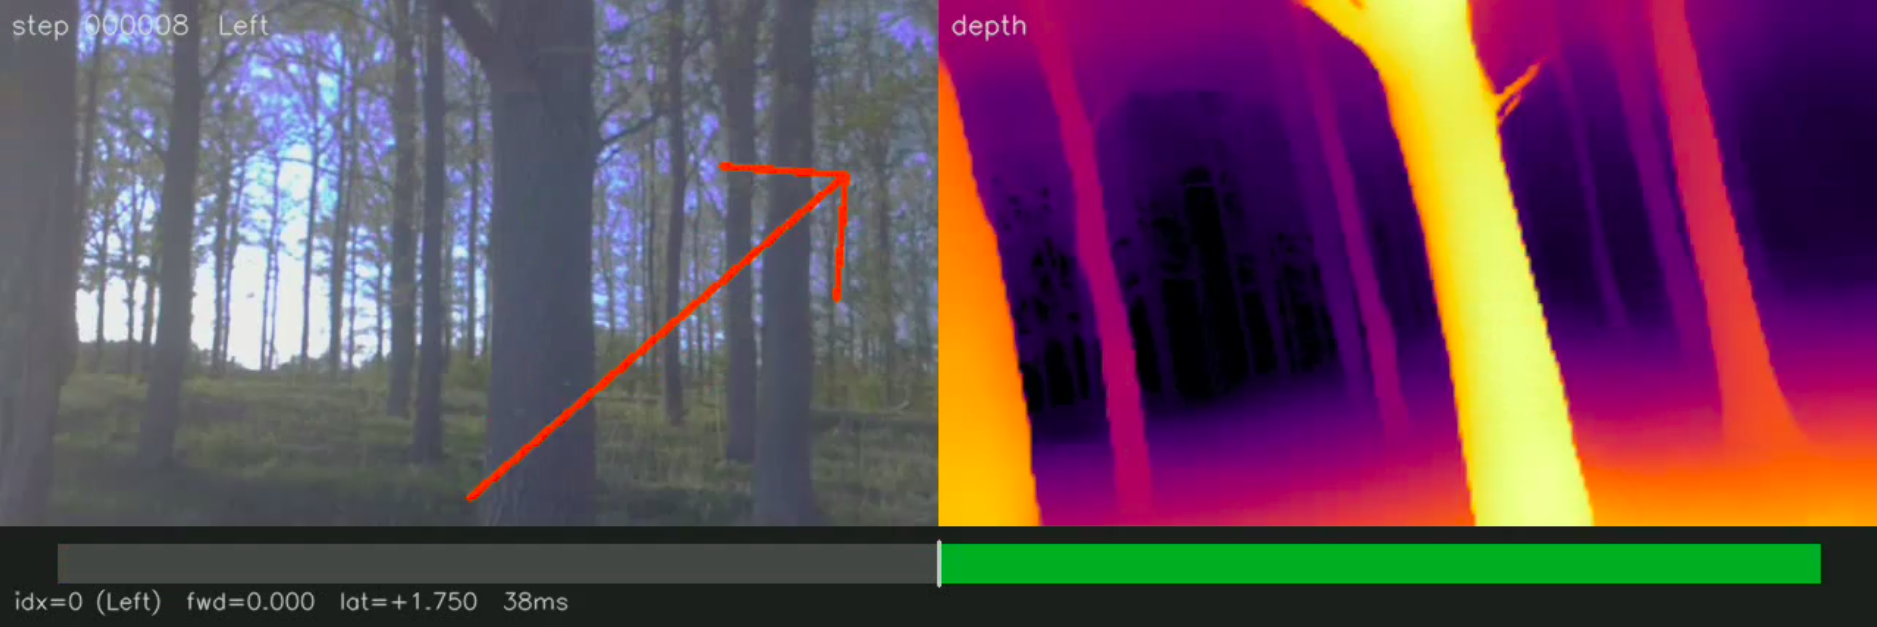
\includegraphics[width=\linewidth]{figures/drone-fpv.png}
    \subcaption{Real first-person view with discrete-action arrow (left/straight/right) and the Depth Anything depth image.}
  \end{minipage}
  \vspace{1cm}
  \caption{First-person view, simulated and real, side by side.}\label{fig:fpv_sxs}
\end{figure}

\begin{figure}[H]
  \centering
  \begin{minipage}[t]{0.48\textwidth}
    \centering
    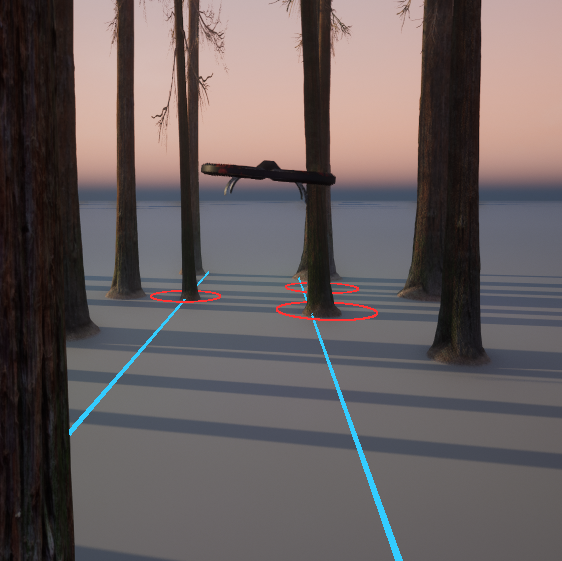
\includegraphics[height=7cm]{figures/sim-drone-flight.png}
    \subcaption{Simulated drone in AirSim.}
  \end{minipage}\hfill
  \begin{minipage}[t]{0.48\textwidth}
    \centering
    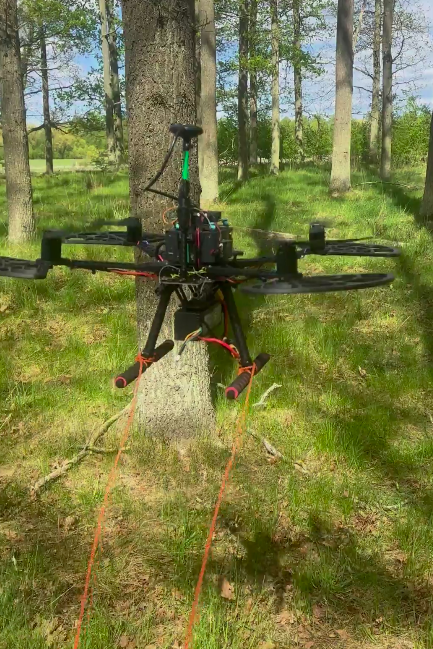
\includegraphics[height=7cm]{figures/drone-flight.png}
    \subcaption{Real Holybro S500 V2 in flight.}
  \end{minipage}
  \vspace{1cm}
  \caption{Drone platform, simulated and real, side by side.}\label{fig:drone_sxs}
\end{figure}

\subsection{Variables}

The same set of variables is logged in simulation and in real flights so the two can be compared directly. For every episode (sparse or dense, simulation or real forest), the following are recorded: the tree density (sparse / dense), the trees in corridor (2 or 3), the trees avoided (0--3), and the episode result (success or fail). The independent variables are \textit{tree density} (sparse, dense) and \textit{environment} (simulation, real forest). The dependent variables, derived from the per-episode log, are the avoidance rate (trees avoided over trees in corridor) and the success rate (successful episodes over total). Drone hardware, camera parameters, control frequency, weather, drone speed, and cruise altitude are treated as control variables and held constant across conditions. The sim-to-real transfer ratio is computed as the real-world success rate divided by the simulation success rate at the matching density. Table~\ref{tab:variables} summarises all variables. The per-episode result tables are listed in the appendix.

\begin{table}[H]
    \small
    \centering
    \vspace*{\baselineskip}
    \caption{Independent, dependent, and control variables. Logged identically in simulation and in the real-world flights.}
    \label{tab:variables}
    \begin{tabular}{p{3cm} p{4cm} p{6cm}}
        \hline\hline
        \rowcolor{lightgray}\textbf{Variable type} & \textbf{Variable} & \textbf{Values / Range} \\\hline
        Independent & Tree density & Sparse (2 trees) / Dense (3 trees) \\
        \rowcolor{lightlightgray} Independent & Environment & Simulation / Real forest \\
        Dependent & Trees avoided & 0--3 (per episode) \\
        \rowcolor{lightlightgray} Dependent & Episode result & Success / Fail \\
        Dependent & Avoidance rate & Trees avoided / Trees in corridor $\times$ 100 \\
        \rowcolor{lightlightgray} Dependent & Success rate & Successful episodes / Total episodes $\times$ 100 \\
        Dependent & Sim-to-real ratio & Real success rate / Sim success rate (per density) \\
        \rowcolor{lightlightgray} Control & Forward cruise speed & 1.0\,m/s \\
        Control & Lateral avoidance speed & 2.0\,m/s \\
        \rowcolor{lightlightgray} Control & Cruise altitude & 1.5\,m \\
        Control & Camera FOV & 62$^{\circ}$ \\
        \rowcolor{lightlightgray} Control & Camera resolution & 126$\times$224\,px \\
        Control & Control frequency & $\sim$10\,Hz \\
        \rowcolor{lightlightgray} Control & Weather conditions & Wind $<$ 3\,m/s, daylight, no precipitation \\
        \hline
    \end{tabular}
\end{table}


\end{document}
